\documentclass[12pt]{article}
\usepackage{polski}
\usepackage[utf8]{inputenc}
\usepackage{graphicx}
\usepackage{amsmath}
\usepackage{graphicx}
\usepackage{setspace}
\usepackage{pdfpages}
\onehalfspacing


\title{ Wyznaczanie przyspieszenia ziemskiego metodą spadku swobodnego \\
    \large Informatyka – profil praktyczny, semestr II \\
    Wydział Matematyki Stosowanej \\
    Politechnika Śląska \\}

\author{ Sekcja 5 \\
    Erwin Matys, Bartłomiej Maliniecki}
\date{Kwiecień 2022}

\begin{document}

\maketitle

\section{Obliczenia i wykresy}

\subsection*{Obliczenie niepewności typu $a$ (statystycznych) średnich czasów
    spadania $u_a(t_{sr})$.} Aby policzyć niepewności typu $a$ skorzystamy ze
wzoru:
\begin{center}
    $u_a(t_{sr}) = \sqrt{\frac{1}{N(N-1)} \displaystyle\sum_{i=1}^{N} (t_i -
            t_{sr})^2} \cdot t_{\alpha, N}$.
\end{center}
Gdzie:
\begin{flushleft}
    $t_{\alpha, N}$ - Współczynnik Studenta Fishera, gdzie za $\alpha$
    przyjmujemy 0.6828, a za $N$ liczbę pomiarów w serii, czyli w naszym
    przypadku 5.
\end{flushleft}
\begin{center}
    $t_{\alpha=0.6828,N=5} = 1.141$
\end{center}
Po uwzględnieniu wszystkich danych wychodzi nam:
\begin{center}
    \begin{tabular} { | c | c | c | }
        \hline
        Lp. & $t_{sr}$, s & $u_a(t_{sr})$, s \\
        \hline
        1.  & 0.31900 & 0.00000 \\ \hline
2.  & 0.34850 & 0.00029 \\ \hline
3.  & 0.37600 & 0.00026 \\ \hline
4.  & 0.40325 & 0.00023 \\ \hline
5.  & 0.42825 & 0.00029 \\ \hline
6.  & 0.45225 & 0.00023 \\ \hline
7.  & 0.47300 & 0.00036 \\ \hline
8.  & 0.49450 & 0.00046 \\ \hline
9.  & 0.51575 & 0.00023 \\ \hline
10. & 0.53400 & 0.00026 \\ \hline
        \hline
    \end{tabular}
\end{center}

\subsection*{Obliczenie niepewności typu $b$ pomiaru czasu $u_b(t)$}
Aby policzyć niepewność typu $b$ pomiaru czaus $u_b(t)$ skorzystamy ze wzoru:
\begin{center}
    $u_b(x) = \frac{\Delta x}{\sqrt{3}}$.
\end{center}
Gdzie $\Delta x = 0.003$ s dla użytego przyrządu.
\begin{center}
    $u_b(t) = \frac{0.003}{\sqrt{3}} = 0.0017$ s.
\end{center}

\subsection*{Obliczenie niepewności całkowitych średnich czasów  \\
    spadania $u(t_{sr})$ i umieszczenie wyników w tabeli}

Do policzenia niepewności całkowitych średnich czasów spadania \\
skorzystamy ze wzoru:
\begin{center}
    $u(t_{sr}) = \sqrt{u_a^2(t_{sr}) + u_b^2(t)}$
\end{center}
Tabelka z danymi:
\begin{center}
    \begin{tabular} { | c | c | c | c | c | }
        \hline
        Lp. & $H$, m & $\sqrt{H}$, $\sqrt{m}$ & $t_{sr}$, s & $u(t_{sr})$, s \\
        \hline
        1.  & 0.500  & 0.707                  & 0.3190     & 0.0017         \\
        \hline
        2.  & 0.600  & 0.775                  & 0.3485      & 0.0018         \\
        \hline
        3.  & 0.700  & 0.837                  & 0.3760      & 0.0018         \\
        \hline
        4.  & 0.800  & 0.894                  & 0.4033      & 0.0017         \\
        \hline
        5.  & 0.900  & 0.949                  & 0.4283      & 0.0018         \\
        \hline
        6.  & 1.000  & 1.0                  & 0.4523      & 0.0017         \\
        \hline
        7.  & 1.100  & 1.049                  & 0.4730      & 0.0018         \\
        \hline
        8.  & 1.200  & 1.095                  & 0.4945      & 0.0018         \\
        \hline
        9.  & 1.300  & 1.14                  & 0.5158      & 0.0017         \\
        \hline
        10. & 1.400  & 1.183                  & 0.5340      & 0.0018         \\
        \hline
    \end{tabular}
\end{center}

\subsection*{Wykres zależności $t_{sr}$ od $H$}

Dla wykresu przyjmujemy następujące niepewności: \\
$u(H) = 0.003$ m \\
$u(t_{sr})$ - Niepewności całkowite średnich czasów spadania.
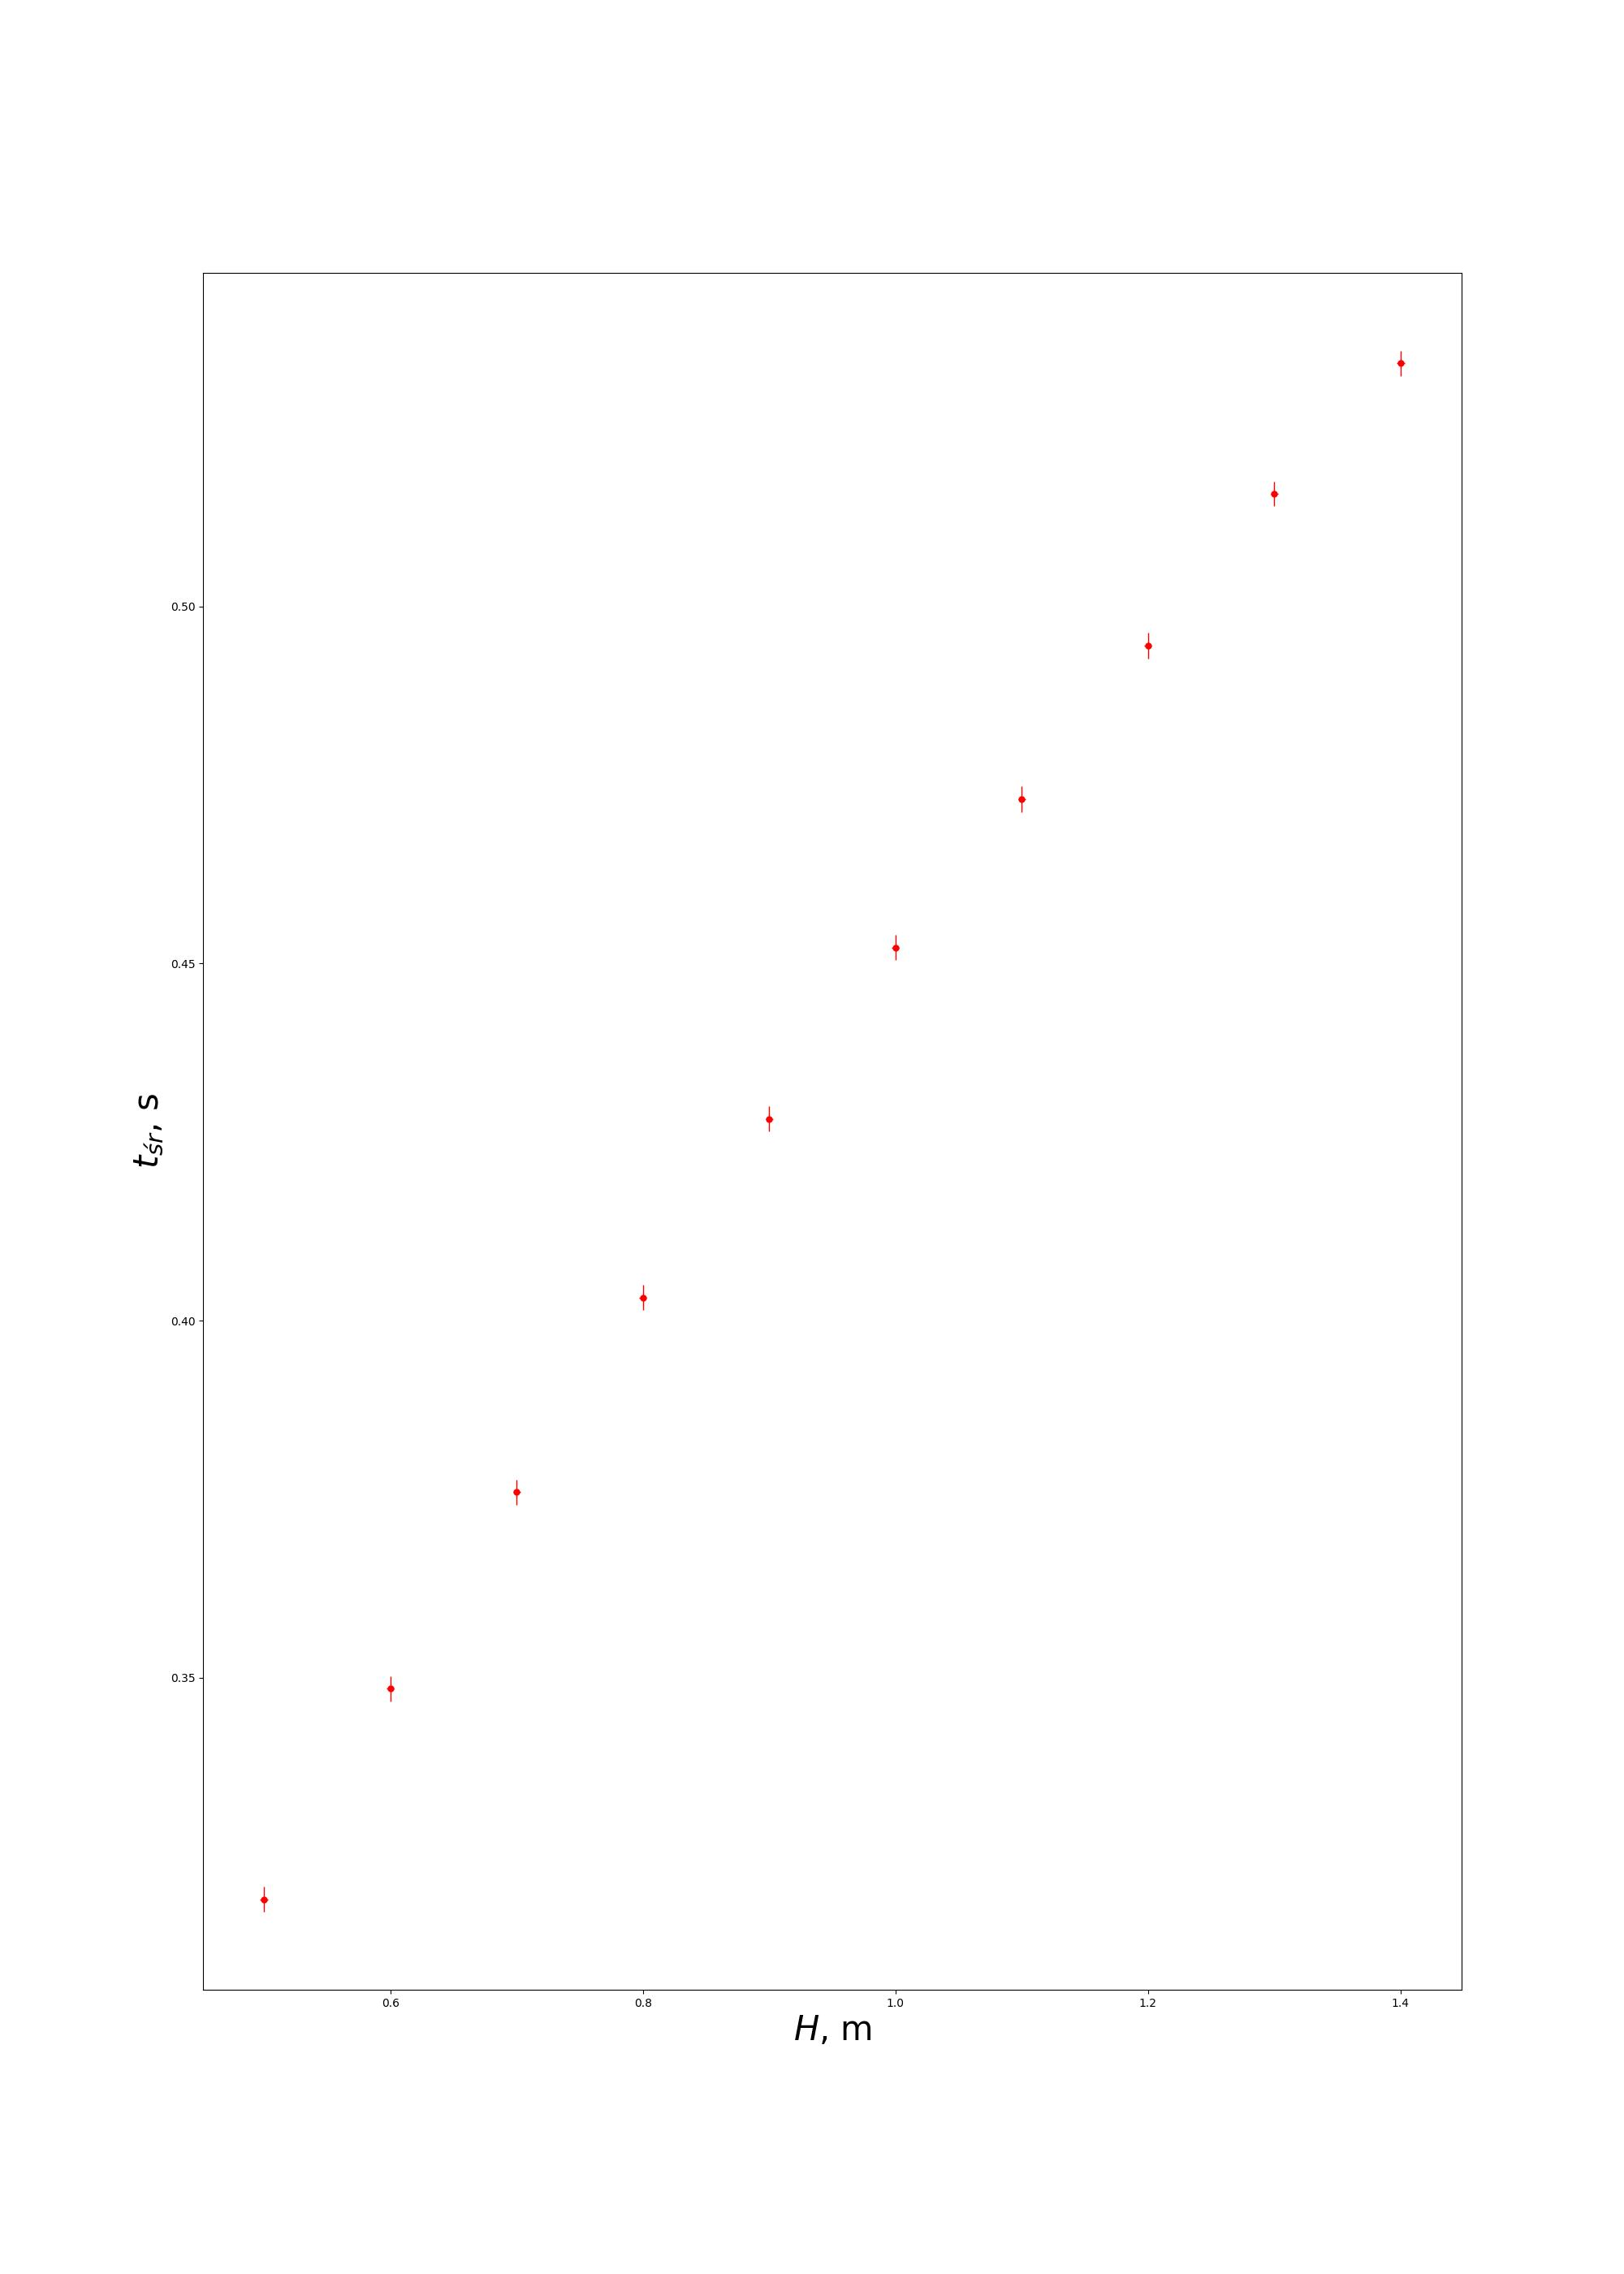
\includepdf{wykres1.jpg}

\subsection*{Wykres zależności $t_{sr}$ od $\sqrt{H}$}

Dla wykresu przyjmujemy następujące niepewności: \\
$u(t_{sr})$ - Niepewności całkowite średnich czasów spadania. \\
Aby policzyć niepewność $u(\sqrt{H})$ musimy użyć prawa przenoszenia
niepewności:
\begin{center}
    $u(y)=\sqrt{\sum_{i=1}^{k}[\frac{\partial y}{\partial x_i}u(x_i)]^2}$.
\end{center}
Dla $y = \sqrt{H}$ równanie ma postać:
\begin{center}
    $u(\sqrt{H}) = \sqrt{[\frac{u(H)}{2\sqrt{H}}]^2} = \frac{u(H)}{2\sqrt{H}}$.
\end{center}
Tabelka z danymi:
\begin{center}
    \begin{tabular} { | c | c | c | }
        \hline
        Lp. & $\sqrt{H}, \sqrt{m}$ & $u(\sqrt{H}), \sqrt{m}$ \\
        \hline
        1.  & 0.7070               & 0.0021                  \\ \hline
        2.  & 0.7750               & 0.0019                  \\ \hline
        3.  & 0.8370               & 0.0018                  \\ \hline
        4.  & 0.8940               & 0.0017                  \\ \hline
        5.  & 0.9490               & 0.0016                  \\ \hline
        6.  & 1.0000              & 0.0015                  \\ \hline
        7.  & 1.0490               & 0.0014                  \\ \hline
        8.  & 1.0950               & 0.0014                  \\ \hline
        9.  & 1.1400               & 0.0013                  \\ \hline
        10. & 1.1830               & 0.0013                  \\ \hline
    \end{tabular}
\end{center}
Wykres na następnej stronie:

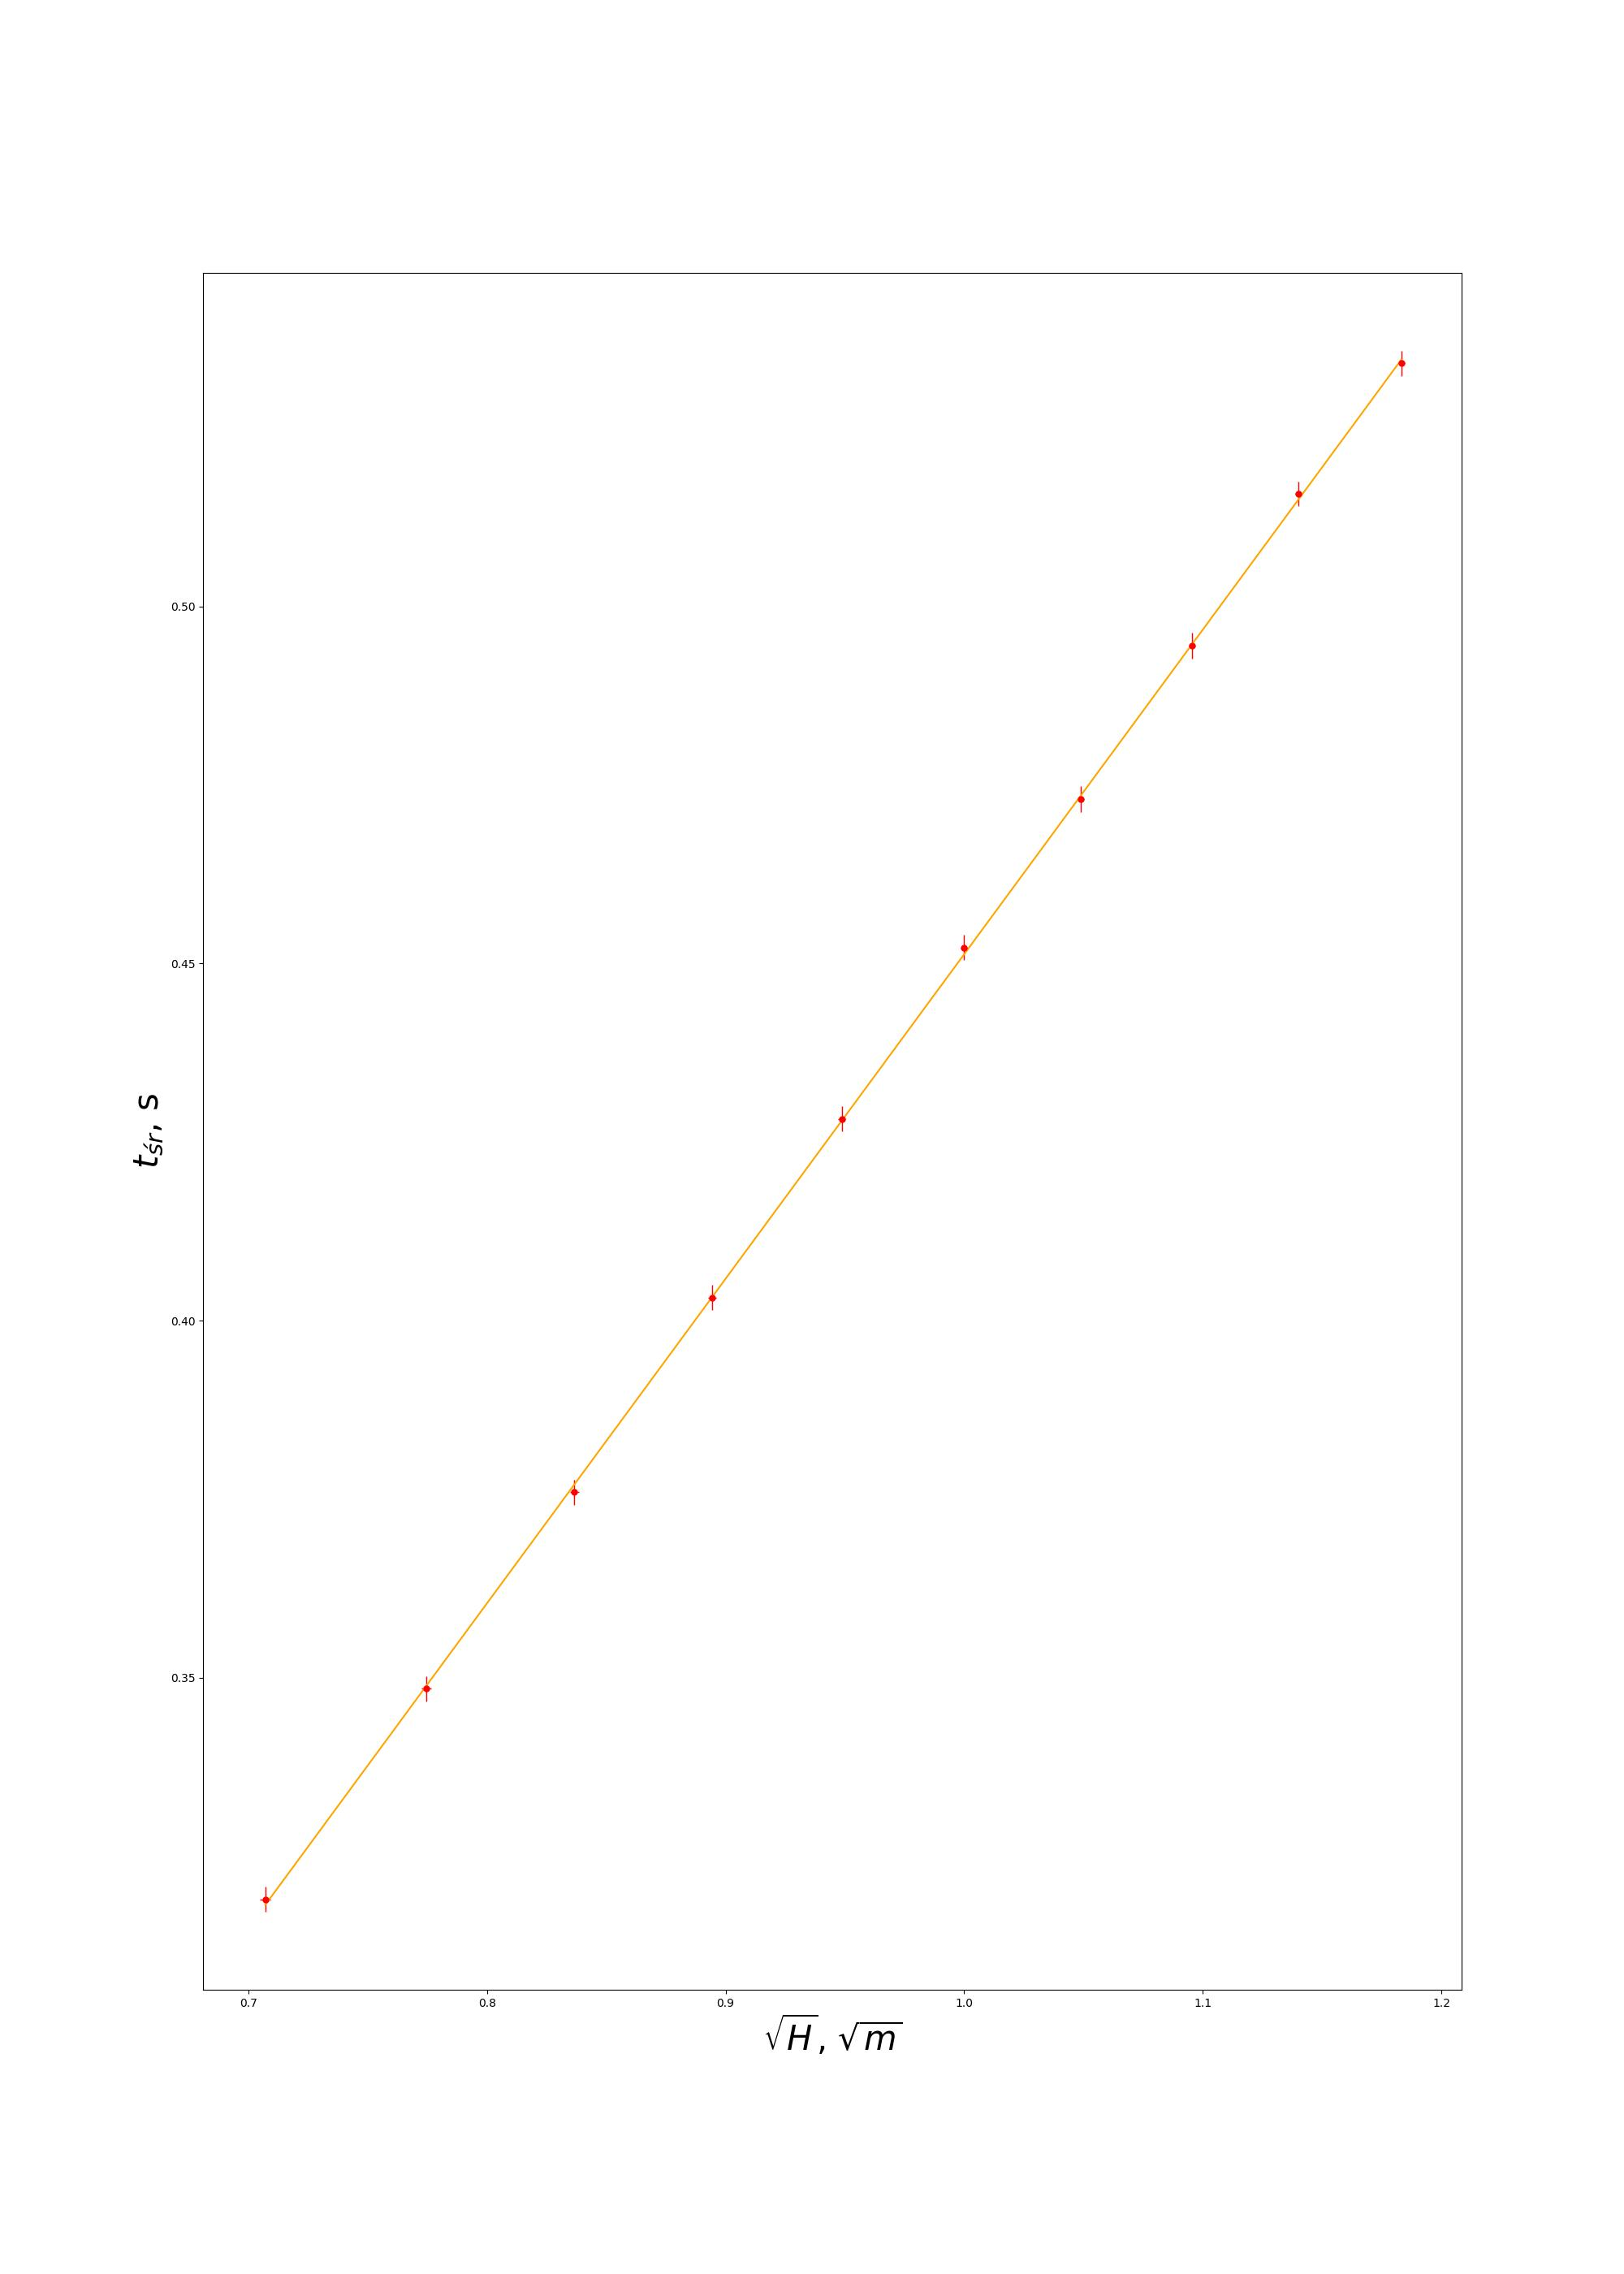
\includepdf{wykres2.jpg}

\subsection*{Wyznaczenie metodą regresji liniowej współczynników prostej
    $t_{sr}(\sqrt{H})$ wraz z niepewnościami}

Aby policzyć współczynniki kierunkowe prostych i wyrazy wolne skorzystamy ze
wzorów:
\begin{flushleft}

    \begin{center}
        $a = \frac{nS_{xy} - S_xS_y}{nS_{xx}-S_x^2}$, $b
            =\frac{S_{xx}S_y-S_xS_{xy}}{nS_{xx}-S_x^2}$
    \end{center}
    Gdzie: \\
    \begin{center}
        $S_x=\displaystyle\sum_{i=1}^{n}x_i$,
        $S_y=\displaystyle\sum_{i=1}^{n}y_i$,
        $S_{xx}=\displaystyle\sum_{i=1}^{n}x_i^2$,
        $S_{xy}=\displaystyle\sum_{i=1}^{n}x_i \cdot y_i$ \\
    \end{center}
\end{flushleft}

\begin{flushleft}
    Do obliczenia niepewności skorzystamy ze wzorów:
    \begin{center}
        $u(a) = \sqrt{\frac{n}{n-2} \cdot
                \frac{S_{\epsilon\epsilon}}{nS_{xx}-S_x^2}}$, $u(b) =
            \sqrt{\frac{1}{n-2} \cdot
            \frac{S_{xx}S_{\epsilon\epsilon}}{nS_{xx}-S_x^2}}$ \\
    \end{center}
    Gdzie: \\
    \begin{center}
        $S_{\epsilon\epsilon}=\displaystyle\sum_{i=1}^{n}\epsilon_i^2$, dla
        $\epsilon_i = y_i - ax_i - b$
    \end{center}

\end{flushleft}

\begin{flushleft}
    Po obliczeniach wartości współczynników są równe:
\end{flushleft}

\begin{center}
    $a = 0.4500\frac{s}{\sqrt{m}}$, \\
    $b = -0.00305$ s.
\end{center}

\begin{flushleft}
    Wartości niepewności współczynników prostej:
\end{flushleft}

\begin{center}
    $u(a) = 0.0015 \frac{s}{\sqrt{m}}$, \\
    $u(b) = 0.00145$ s.
\end{center}
Postać końcowa:
\begin{center}
    $a = 0.4500(15)\frac{s}{\sqrt{m}}$, $b = -0.00305(145)$ s
\end{center}
\subsection*{Wyznaczenie przyspieszenia ziemskiego $g$}

Aby wyprowadzić wzór na przyspieszenie ziemskie skorzystamy z równania na drogę
w ruchu jednostajnie przyspieszonym:
\begin{center}
    $ S = S_{0} + v_{0}t + \frac{1}{2}at^2$
\end{center}
Przyjmując $S_{0} = 0$ i $v_{0} = 0$ oraz zamieniając drogę $S$ na wysokość $H$
i przyspieszenie $a$ na przyspieszenie ziemskie $g$ otrzymujemy:
\begin{center}
    $H = \frac{1}{2}gt^2$
\end{center}
Przekształcając wzór, w celu wyznaczenia $g$:
\begin{center}
    $g = \frac{2H}{t^2}$
\end{center}
Współczynnik kierunkowy funkcji $t_{sr}(\sqrt{H})$ jest równy $a =
    \frac{t_{sr}}{\sqrt{H}}$. Możemy to $a$ podstawić do wzoru na $g$ i
otrzymujemy:
\begin{center}
    $g = \frac{2}{a^2}$
\end{center}
Po wstawieniu odpowiednich danych otrzymujemy:
\begin{center}
    $g = \frac{2}{0.45^2} = 9.88 \frac{m}{s^2}$
\end{center}

\subsection*{Obliczenie niepewności przyspieszenie ziemskiego $g$ \\
    korzystając z prawa przenoszenia niepewności}

Aby wyliczyć niepewność przyspieszenia ziemskiego $g$, skorzystamy z prawa
przenoszenia niepewności. Przyjmujemy, że niepewność $u(a) = 0.0015
    \frac{s}{\sqrt{m}}$. Prawo przenoszenia niepewności wyraża się wzorem:
\begin{center}
    $u(y) = \sqrt{\sum_{i=1}^{k}[\frac{\partial y}{\partial x_i}u(x_i)]^2}$
\end{center}
Zatem prawo przenoszenia niepewności dla $g$ ma postać:
\begin{center}
    $u(g) = \sqrt{(\frac{-4}{a^3} \cdot u(a))^2}$
\end{center}
Po wstawieniu liczb:
\begin{center}
    $u(g) = 0.066 \frac{m}{s^2}$
\end{center}

\subsection*{Obliczenie niepewności rozszerzonej}
Aby policzyć niepewność rozszerzoną skorzystamy ze wzoru:
\begin{center}
    $U(y) = k \cdot u(y)$.
\end{center}
Gdzie: \\
\indent $k$ - bezwymiarowy współczynnik rozszerzenia. Przyjmujemy $k=2$. \\
\indent $u(y)$ - niepewność badanej wartości. \\
Dla $g$:
\begin{center}
    $U(g) = 2 \cdot u(g) = 0.13 \frac{m}{s^2}$. \\
    $g = 9.88 \pm 0.13 \frac{m}{s^2}$.
\end{center}
\subsection*{Obliczenie przyspieszenia ziemskiego dla Gliwic i \\
    porównanie wyniku z otrzymaną wartością}

Aby policzyć przyspieszenie ziemskie dla danej szerokości geograficznej i
wysokości nad poziomem morza, skorzystamy ze wzoru:
\begin{center}
    $g_{\varphi} \approx 9.780318(1+0.0053024\sin^2\varphi -
        0.0000058\sin^22\varphi)-3.086 \cdot 10^{-6}h$
\end{center}
Gdzie: \\
\indent $\varphi$ - szerokość geograficzna [$^{\circ}$], \\
\indent $h$ - wysokość nad poziomem morza [m]. \\
Przyjmując szerokość geograficzną $\varphi = 50.3^{\circ}$ i wysokość nad
poziomem \\
morza $h = 219$ m otrzymujemy:
\begin{center}
    $g_0 = 9.80 \frac{m}{s^2}$.
\end{center}
Przeprowadzimy test zgodności otrzymanego $g$ w wyniku doświadczenia z
przyspieszeniem ziemskim $g_0$ dla Gliwic: \\
Test zgodności ma postać:
\begin{center}
    $|y - y_0| < U(y)$ \\
\end{center}
Wstawiając $g$ i $g_0$:
\begin{center}
    $|g - g_0| < U(g)$ \\
    $ 0.08 < 0.132 $
\end{center}
Co pokazuje, że test zgodności zachodzi dla $g$ zmierzonego przez nas.

\section{Wnioski}

Otrzymane wyniki potwierdziły poprawność wzoru na czas spadku swobodnego.

Co prawda doświadczenia nie wykonaliśmy w próżni, ale masa naszej kulki była na
tyle duża, a jej rozmiar i odległość z jakiej ją zrzucaliśmy na tyle małe, a że
mogliśmy zaniedbać opory powietrza.

\end{document}
